\definecolor{okblue}{HTML}{0072B2}\definecolor{okorange}{HTML}{E69F00}\definecolor{okverm}{HTML}{D55E00}\definecolor{okgrey}{HTML}{999999}
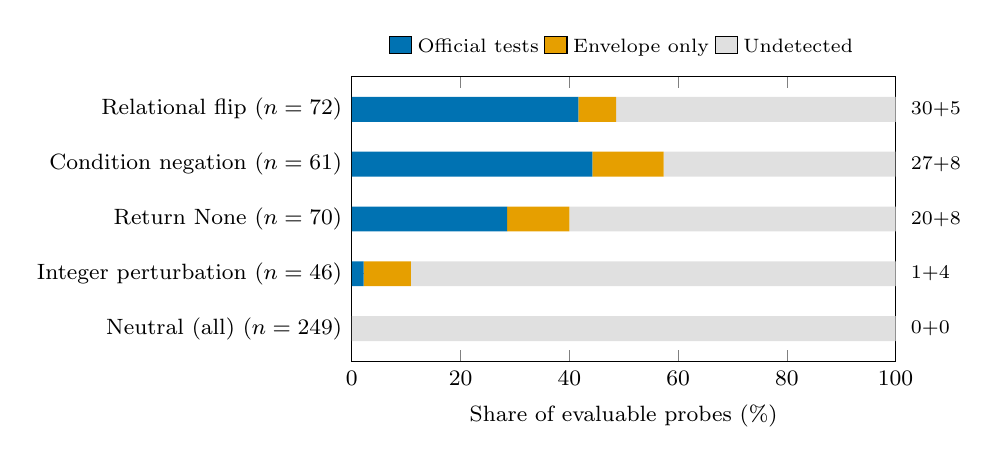
\begin{tikzpicture}
\begin{axis}[xbar stacked,bar width=9pt,width=0.70\linewidth,height=52mm,xmin=0,xmax=100,
 ymin=0.4,ymax=5.6,y dir=reverse,ytick={1,2,3,4,5},yticklabels={{Relational flip ($n=72$)},{Condition negation ($n=61$)},{Return \code{None} ($n=70$)},{Integer perturbation ($n=46$)},{Neutral (all) ($n=249$)}},
 xlabel={Share of evaluable probes (\%)},tick label style={font=\footnotesize},label style={font=\footnotesize},
 legend style={font=\scriptsize,at={(0.5,1.03)},anchor=south,legend columns=3,draw=none},clip=false]
\addplot[fill=okblue,draw=none] coordinates {(41.67,1) (44.26,2) (28.57,3) (2.17,4) (0.00,5)};
\addlegendentry{Official tests}
\addplot[fill=okorange,draw=none] coordinates {(6.94,1) (13.11,2) (11.43,3) (8.70,4) (0.00,5)};
\addlegendentry{Envelope only}
\addplot[fill=black!12,draw=none] coordinates {(51.39,1) (42.62,2) (60.00,3) (89.13,4) (100.00,5)};
\addlegendentry{Undetected}
\node[anchor=west,font=\scriptsize] at (axis cs:101,1) {30+5};
\node[anchor=west,font=\scriptsize] at (axis cs:101,2) {27+8};
\node[anchor=west,font=\scriptsize] at (axis cs:101,3) {20+8};
\node[anchor=west,font=\scriptsize] at (axis cs:101,4) {1+4};
\node[anchor=west,font=\scriptsize] at (axis cs:101,5) {0+0};
\end{axis}
\end{tikzpicture}
